\documentclass[11pt]{article}
\usepackage[a4paper,margin=2.35cm]{geometry}
\usepackage{amsmath,amssymb,amsthm,booktabs,graphicx,float,array,microtype}
\usepackage[colorlinks=true,allcolors=blue]{hyperref}
\usepackage[font=small,labelfont=bf]{caption}
\usepackage{enumitem}
\newcommand{\doublespacing}{\renewcommand{\baselinestretch}{2}\selectfont}
\graphicspath{{../figures/}}
\newtheorem{proposition}{Proposition}
\newtheorem{theorem}{Theorem}
\newtheorem{corollary}{Corollary}
\newcommand{\nrmse}{\operatorname{NRMSE}}
\newcommand{\indet}{\textsc{Indeterminate}}
\title{Power-Certified Model-Order Selection with Abstention\\for Sparse Multichannel Transient Signals}
\author{Haitao Duan$^{1}$, Ning Hu$^{2,*}$, Shuqun Li$^{3}$, Chuyang Hu$^{4}$\\[2mm]
\small $^1$School of Computer Science, Hangzhou Dianzi University, Hangzhou, China\\
\small $^2$School of Mechanical Engineering, Hangzhou Dianzi University, Hangzhou, China\\
\small $^3$School of Mathematics and Physics, Xi'an Jiaotong-Liverpool University, Suzhou, China\\
\small $^4$Department of Computer Science and Engineering,\\
\small University of California, Santa Cruz, CA 95064, USA\\[1mm]
\small $^*$Corresponding author: \href{mailto:huning@hdu.edu.cn}{huning@hdu.edu.cn}}
\date{}

\begin{document}
\doublespacing
\maketitle

\begin{abstract}
Finite sums of decaying modes are routinely used to represent hereditary dynamics, yet a good fit does not establish that the inferred modes are identifiable or transferable. This paper develops an evidence-gated protocol for selecting the smallest shared finite memory realization supported by sparse multichannel observations and for refusing a mechanistic rank claim when predictive adequacy and identifiability disagree. Positive rates are shared across independent experimental units, whereas amplitudes and offsets remain unit specific. Candidate ranks are evaluated jointly by information gain, held-unit early-to-late prediction, cross-fold rate stability, and adjacent-rate separation. A Gaussian two-point theorem establishes an adjacent-rate indistinguishability boundary, while a separate corollary states explicit conditions for a calibrated refusal gate. A threshold calibrated on disjoint semi-synthetic data separates well-resolved and coalesced controls in 40 of 40 trials under each of four noise generators; the per-generator Wilson 95\% lower bound is 0.9124, so this remains design-conditional rather than universal evidence. In a separate 1,080-trial finite-budget atlas, block matrix-pencil BIC selected rank two 157 times, including 60 inaccurate rate recoveries; adding separation, local-information, and cross-pencil stability gates retained 74 supported recoveries and no inaccurate one. On a disjoint 1,152-trial common-budget evaluation, a design-power certificate yields 0.2943 coverage and 0.1386 selective risk with zero false order elevation, whereas five full-coverage matrix-pencil, block-Hankel, and Prony criteria expose different elevation--reduction tradeoffs. Four independent public domains provide complementary tests. Full-horizon PVA stress relaxation supports a rank-three finite empirical realization, and 17 copper-alloy stress-relaxation tests across nine material groups support a shared rank-one empirical realization under AR(1)-profile BIC. Gas-sensor recovery predicts well with rank three but contains coalesced rates and is therefore indeterminate. Hydraulic cooling transients improve ordinary BIC but fail held-state transfer. Retrospective transfer of the frozen common-budget rule admits only one of 56 cross-task groups; all 84 overlapping six-of-nine PVA subsets remain admissible and reject rank-one sufficiency. The study separates predictive improvement, finite representation, and mechanism identification, and provides a versioned Python interface and machine-readable decision records.
In a preregistered first P5 application to six cable-ageing curves, the unchanged rule admits the group and rejects rank-one sufficiency; prior use of the data in another project prevents calling this prospective acquisition.
\end{abstract}

\noindent\textbf{Keywords:} statistical signal processing; detection and estimation; model-order selection;\\
spectral resolution; selective inference; multichannel transient signals

\section{Introduction}
Hereditary systems are often compressed into finite sums of exponentials. Such representations connect relaxation spectra, rational approximations, auxiliary-state models, and non-Markovian reduced dynamics. Classical Prony recovery and vector fitting provide effective reconstruction machinery \cite{stampfer2020gop,gustavsen1999vector,bosner2021parallel}, while recent generalized Langevin models learn increasingly expressive memory kernels from trajectories \cite{lei2016parameterization,ge2024state,lang2026learning}. The central question addressed here is different: when do finite, noisy, grouped observations support a particular minimal shared realization, and when should the analysis refuse to assign a mechanistic rank?

Selecting the curve with the smallest residual is insufficient. Additional modes can absorb noise, closely spaced rates can become locally indistinguishable, and a model that predicts held observations can still contain an unresolved internal spectrum. These problems are amplified when channels from the same experiment are treated as independent replicates or when the observed window does not reach the asymptotic tail. Consequently, model support must combine fit, transfer, stability, and separability rather than rely on one score.

We introduce a joint identification-and-refusal protocol with four contributions. First, it defines a shared-rate, unit-specific-amplitude model and selects the smallest rank that passes four predeclared evidence gates. Second, it adds an explicit \indet{} outcome so predictive gains cannot be promoted automatically to a mechanism claim. Third, it maps observation-design boundaries and relates them to residual correlation and the conditioning of rate sensitivities. Fourth, it implements the protocol as a versioned software contract with stable \texttt{fit}, \texttt{evaluate}, \texttt{decide}, and \texttt{report} operations.

Public PVA and copper-alloy relaxation, gas-sensor, and hydraulic datasets test transfer across specimens, material groups, batches, and component states \cite{schelkow2026pva,kupferdigital2024relaxation,ziyatdinov2015dataset,ziyatdinov2015bioinspired,helwig2018hydraulic}. Two supported realizations and two different refusals distinguish identified structure from favorable fit. A fifth cable-ageing dataset supplies a preregistered new-to-P5 frozen-rule transfer \cite{kayanja2026cableageing}; prior P3 analysis precludes describing it as investigator-blind or prospectively acquired.

\section{Related work and contribution boundary}
Finite exponential and rational representations have a long numerical history. Generalized Prony methods recover sparse eigenfunction expansions and analyze reconstruction sensitivity \cite{stampfer2020gop}; matrix-pencil variants extend recovery to multivariate observations \cite{bosner2021parallel}; and vector fitting estimates shared poles from frequency-domain responses \cite{gustavsen1999vector}. We use these ideas as representation and baseline machinery. We do not propose a new Prony solver or claim exact recovery from noisy data.

In data-driven non-Markovian modeling, rational auxiliary-state parameterizations and learned memory kernels support accurate reduced dynamics \cite{lei2016parameterization,ge2024state,lang2026learning}. Their primary objective is kernel estimation or dynamical prediction. Our objective is an evidence decision about the minimum finite realization shared across independent units, including a refusal when the data cannot separate candidate mechanisms.

Our earlier DFSC work makes a differentiable Mittag--Leffler propagator available as a SciML primitive \cite{hu2026dfsc}. That contribution concerns differentiable propagation, numerical control, and software composition. The present work neither extends that evaluator nor uses its implementation as the source of the statistical claim; it addresses a distinct inference problem: whether grouped observations identify a shared finite memory realization at all. This boundary prevents software availability from being mistaken for mechanism identifiability.

Relaxation-spectrum identification is also established in viscoelasticity, where regularization and time-scale selection stabilize inverse recovery \cite{stankiewicz2023relaxation}. Closely spaced exponential nodes are intrinsically ill-conditioned through their Vandermonde geometry \cite{moitra2015superresolution}; this motivates a refusal option rather than forced order selection. Classical BIC and small-sample time-series corrections further show why parameter count and residual dependence must be separated \cite{schwarz1978bic,hurvich1989timeseries}. The present protocol complements these estimators by requiring held-unit prediction, foldwise rate stability, and rate separation. Its novelty is therefore the joint decision contract, not any individual constituent criterion.
Classical model-order research distinguishes information-criterion evidence, predictive selection, and Bayesian evidence rather than treating them as equivalent \cite{stoica2004modelorder,shao1993crossvalidation,kass1995bayes}. Selective prediction likewise formalizes abstention when a requested risk cannot be supported \cite{geifman2017selective}. Our refusal differs in object: it abstains from a shared dynamical-rank interpretation, not from an individual class prediction. This literature motivates the explicit decision state, while the four-gate grouped dynamical audit is specific to the present problem.

\section{Model and evidence contract}
\subsection{Shared finite realization}
For experimental unit $i$ observed at times $t_{ij}$, the candidate rank-$r$ model is
\begin{equation}
y_i(t)=c_i+\sum_{k=1}^{r}a_{ik}\exp(-\lambda_k t)+\varepsilon_i(t),
\qquad a_{ik}\in\mathbb R,\quad 0<\lambda_1<\cdots<\lambda_r.
\label{eq:model}
\end{equation}
The rates $\lambda_k$ are shared across units; amplitudes $a_{ik}$ and offsets $c_i$ are unit specific. This factorization separates a candidate common spectrum from experimental scale and baseline differences. It is appropriate only on a declared interval where positive finite exponential relaxation is a plausible representation.

\subsection{Four evidence gates}
Candidate ranks $r=1,\ldots,r_{\max}$ are fitted using training units. The smallest rank is supported only if it passes all four gates.

\paragraph{Information gate.} Let $n$ be the number of fitted observations and $q_r$ the number of free parameters. We use the independent-residual score
\begin{equation}
\mathrm{BIC}_r=n\log(\mathrm{SSE}_r/n)+q_r\log n,
\end{equation}
and require a predeclared improvement over the lower rank \cite{schwarz1978bic}. Because relaxation residuals are serially correlated, every final audit additionally reports a Gaussian AR(1) profile-BIC and an effective sample-size diagnostic. Agreement is supporting evidence; disagreement triggers sensitivity reporting rather than retrospective threshold selection \cite{hurvich1989timeseries}.


\paragraph{Transfer gate.} Complete experimental units are held out. Rates are learned from the remaining units, amplitudes are calibrated on the first 60\% of the held curve, and the final 40\% is predicted. Error is summarized by
\begin{equation}
\nrmse_i=\frac{\|\hat{\mathbf y}_{i,\mathrm{late}}-\mathbf y_{i,\mathrm{late}}\|_2}
{\|\mathbf y_{i,\mathrm{late}}-\bar y_{i,\mathrm{late}}\mathbf 1\|_2+\epsilon}.
\end{equation}

\paragraph{Stability gate.} Foldwise log-rates must remain sufficiently stable. For each mode, the standard deviation of $\log\lambda_k$ across held-unit folds must not exceed a frozen tolerance.

\paragraph{Separation gate.} Adjacent rates must satisfy
\begin{equation}
\min_k\frac{\lambda_{k+1}}{\lambda_k}\ge \rho_{\min}>1.
\label{eq:separation}
\end{equation}
This prevents a numerically improved but coalesced spectrum from being interpreted as distinct timescales.

If no rank passes all gates, the output is \indet{}. This is not an optimization failure: it records that the declared observations do not support the requested mechanism-level resolution.

\begin{figure}[H]
\centering
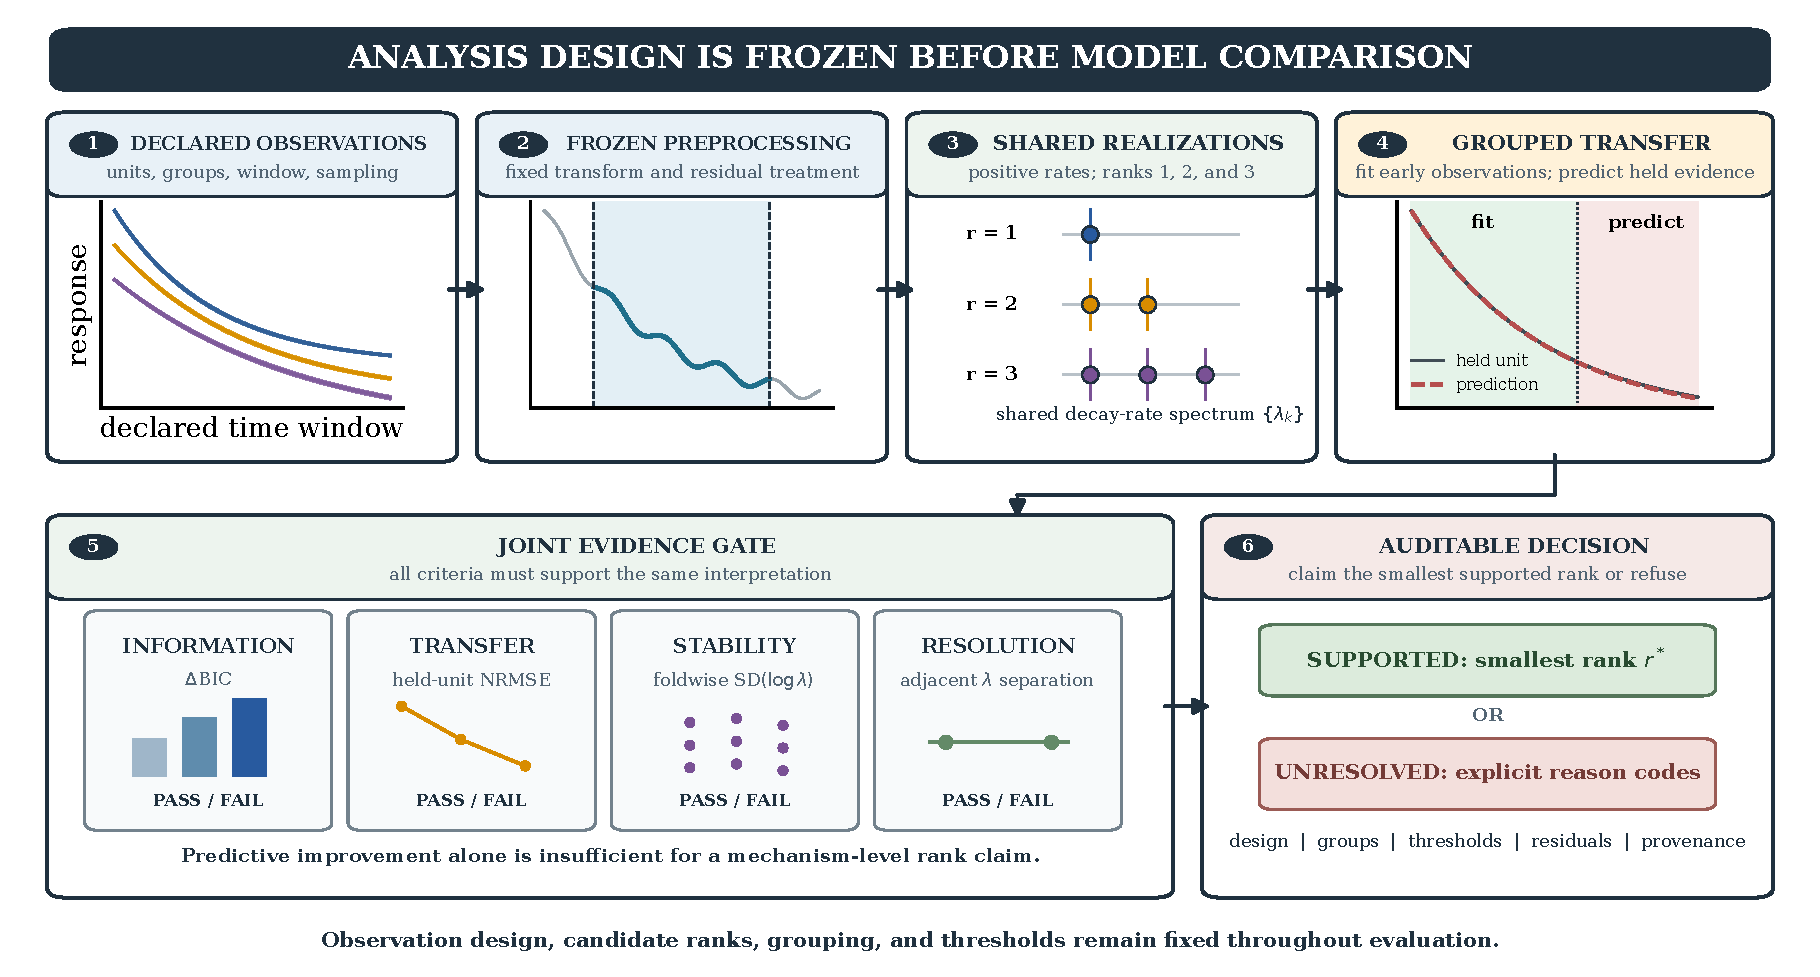
\includegraphics[width=0.96\textwidth]{fig_stage62_method_workflow.pdf}
\caption{Frozen analysis workflow. Decisions are made at the level of independent experimental units, not individual channels or repeated samples.}
\label{fig:workflow}
\end{figure}

\subsection{Minimal identifiability analysis}
Let $\boldsymbol\mu(\theta)$ stack the mean responses and let $J=\partial\boldsymbol\mu/\partial\theta$. Local identification requires that the rate-related columns of $J$ remain linearly independent after nuisance amplitudes and offsets are projected out.

\begin{proposition}[Local rate identification]
If the projected rate-sensitivity matrix $J_\lambda$ has full column rank at $\theta^\star$, then the shared rates are locally identifiable in a neighborhood of $\theta^\star$. If its smallest singular value tends to zero, local uncertainty diverges and distinct nearby rates cannot be stably resolved.
\end{proposition}
\begin{proof}
Full column rank makes the local Fisher/Gauss--Newton matrix $J_\lambda^\top WJ_\lambda$ positive definite for positive definite $W$. The inverse-function argument gives local injectivity. Vanishing smallest singular value makes the inverse sensitivity unbounded.
\end{proof}

For two close rates $\lambda$ and $\lambda+\delta$, the mean-value theorem gives
\begin{equation}
|e^{-\lambda t}-e^{-(\lambda+\delta)t}|
\le |\delta|t e^{-\min(\lambda,\lambda+\delta)t}.
\label{eq:coalescence}
\end{equation}
Thus a finite noisy window may not distinguish the pair even when the two-mode fit lowers residual error. Equation~\eqref{eq:coalescence} motivates the separation gate, while the singular spectrum of $J_\lambda$ supplies a continuous diagnostic.

Raw sample count alone is not an information measure. Under correlated residuals with covariance $\Sigma$, local information is $J^\top\Sigma^{-1}J$. Extending the horizon changes the sensitivity geometry and residual correlation simultaneously; denser sampling can add nearly redundant rows. Support boundaries therefore need not be monotone in sample count.

The adjacent-rate limit can be stated formally. Consider independent Gaussian observations with variance $\sigma^2$ and an alternative containing $a_i e^{-\lambda t}+b_i e^{-(\lambda+\delta_n)t}$. Its merged lower-rank comparison uses $(a_i+b_i)e^{-\lambda t}$. Define
\begin{equation}
R_n^2=\frac{\delta_n^2}{\sigma^2}\sum_{i,\ell}b_i^2t_{i\ell}^2
e^{-2\min(\lambda,\lambda+\delta_n)t_{i\ell}}.
\label{eq:boundary-index}
\end{equation}

\begin{theorem}[Gaussian adjacent-rate indistinguishability]
Under the declared Gaussian model, $\mathrm{KL}(P_{r,n}\|P_{r-1,n})\le R_n^2/2$. If $R_n\to0$, every measurable rank test obeys $\alpha_n+\beta_n\to1$; hence no uniformly consistent rank decision exists along this sequence.
\end{theorem}
\begin{proof}
The mean difference is $d_{i\ell}=b_i[e^{-(\lambda+\delta_n)t_{i\ell}}-e^{-\lambda t_{i\ell}}]$. Equation~\eqref{eq:coalescence} bounds $\|d\|_2^2/\sigma^2$ by $R_n^2$. The common-covariance Gaussian formula gives the KL bound. Pinsker's inequality and the two-point testing bound yield $\alpha_n+\beta_n\ge1-\operatorname{TV}(P_{r,n},P_{r-1,n})\ge1-R_n/2$ \cite{tsybakov2009nonparametric}.
\end{proof}

\begin{corollary}[Embedded multi-rate obstruction]
Suppose all nuisance components and all rates except one adjacent pair are fixed or estimated with error $o(R_n)$. The rank-$r$ and merged rank-$(r-1)$ classes then contain the two-point subexperiment of the theorem. Consequently, if $R_n\to0$, no test can be uniformly consistent over the larger classes.
\end{corollary}
\begin{proof}
Restrict the larger parameter spaces to the two distributions used in the theorem. Uniform consistency on the larger spaces would imply consistency on this restricted pair, contradicting the theorem.
\end{proof}
\begin{corollary}[Conditional consistency of a calibrated refusal gate]
Let $\widehat D_n$ be a diagnostic and $c_n$ a threshold calibrated independently of the evaluation sample. If $\widehat D_n/c_n\stackrel{p}{\to}0$ on an unresolved sequence and $\widehat D_n/c_n\stackrel{p}{\to}\infty$ under a fixed separated, locally identifiable rank, then the rule that refuses when $\widehat D_n\le c_n$ refuses the former and passes the diagnostic gate for the latter with probability tending to one. Acceptance of the true rank additionally requires consistency of the information, transfer, and stability gates.
\end{corollary}

These results are local or embedded statements. They do not establish global identifiability for unrestricted nonlinear kernels, irregular designs, non-Gaussian noise, or jointly drifting nuisance parameters. The implementation reports a local proxy $\widehat D$: log-rate sensitivities are projected off curve-specific offset and amplitude columns, and the smallest projected singular value is multiplied by the minimum adjacent log-rate gap and divided by residual noise. Division by the square root of the observation count removes its leading sample-size scaling. Neither version is an estimator of $R_n$ without additional assumptions. We therefore calibrate the normalized proxy on a declared semi-synthetic design and evaluate it on disjoint seeds; it remains a task-internal diagnostic rather than a universal threshold.

\subsection{Declared extensions beyond positive fully shared rates}
We additionally test four scoped extensions without changing the frozen decisions on the four public datasets. Stable oscillatory memory is represented by real conjugate-pole blocks,
\begin{equation}
y_i(t)=c_i+\sum_k a_{ik}e^{-\lambda_k t}+\sum_j e^{-\gamma_j t}\{u_{ij}\cos(\omega_jt)+v_{ij}\sin(\omega_jt)\}+\epsilon_i(t),
\label{eq:oscillatory-extension}
\end{equation}
where $\gamma_j,\omega_j>0$. Partial sharing uses $\log\lambda_{gk}=\mu_k+\delta_{gk}$ with $\sum_g\delta_{gk}=0$ and a declared quadratic penalty $\eta\sum_{g,k}\delta_{gk}^2$; $\eta$ must be selected without the final evidence group. A dense log-normal relaxation measure supplies an out-of-class stress test of the finite-sum assumption. Finally, a group-level conformal audit uses one nonconformity score per independent calibration group. For $m$ exchangeable calibration groups, its upper threshold is the $\lceil(m+1)(1-\alpha)\rceil$-th order statistic (capped at $m$), and the upper-tail test value is $(1+\#\{S_j\ge S_{\rm test}\})/(m+1)$ \cite{shafer2008conformal}. This is a finite-sample marginal statement under group exchangeability, not a distribution-free guarantee after group shift.
\section{Public datasets and frozen protocols}
\subsection{PVA stress relaxation}
The first task uses the public stress-relaxation dataset of cylindrical PVA gel polymer electrolyte samples \cite{schelkow2026pva}. It contains three specimens and three cycles per specimen. No smoothing is applied. Rates are learned with leave-one-specimen-out folds, and the complete 28-s task contains 96 retained points per curve. Because only three specimens are independent, curve-level uncertainty summaries are descriptive and are not treated as population-level inference.

\subsection{Copper-alloy stress relaxation}
The second task uses the public KupferDigital mechanical-testing archive \cite{kupferdigital2024relaxation}. Seventeen physical stress-relaxation test files from nine material-code groups are treated as independent experimental units. Engineering stress is divided by the first registered stress, and each curve is registered without smoothing on a common 96-point grid from zero to the shortest complete endpoint within the declared 24-hour tests. Complete material-code groups are held out, so repeated specimens from one group never cross a fold. The decision concerns a shared empirical relaxation realization and is not evidence for a unique microscopic mechanism.

\subsection{Gas-sensor recovery}
The third task uses UCI dataset 308 \cite{ziyatdinov2015dataset}. Fifty non-air exposure experiments are retained from five acquisition batches. Each experiment contains 16 metal-oxide sensor channels. The analysis is restricted to the registered 180--300 s recovery interval, summarized by medians over the physical 12-s modulation cycle. Channels remain clustered within an exposure, and complete acquisition batches are held out. Thresholds and the 60/40 calibration/prediction split are frozen before fitting.

\subsection{Hydraulic cooling transients}
The fourth task uses UCI dataset 447, acquired from a hydraulic test rig over repeated 60-s load cycles \cite{helwig2018hydraulic}. It is an external multichannel dynamic stress test selected for repeated controlled states and clustered sensors; it is not presented as validation of a component-level relaxation mechanism. Valve condition, pump leakage, accumulator pressure, and the stability flag are fixed; cooler efficiency varies over 3\%, 20\%, and 100\%. Ten independent cycles are retained per state. Four channels (cooling efficiency, cooling power, and two temperatures) are analyzed over seconds 20--55 without smoothing. Normalization uses only the first 22 samples of the declared window. Complete cooler states are held out, and channels remain clustered within their cycle.

\subsection{Preregistered cable-ageing transfer}
The fifth source contains unaged and compression-aged stress-relaxation curves for hard, soft, and semiconductive silicone rubber used in cable accessories \cite{kayanja2026cableageing}. Before revealing the P5 outcome, the workbook hash, six named curves, extraction coordinates, and unchanged Stage 69/72 thresholds were frozen. Each curve has at least 2,757 raw observations; the common adapter retains six channels on 24 normalized points. Because P3 had already analysed the raw data for a different question, this is new-to-P5 transfer rather than prospective acquisition.

\subsection{Baselines and statistical audits}
The gas task compares the shared-rate model with independent nonlinear rank-three fitting, fixed-grid nonnegative least squares (NNLS), and a Prony recurrence baseline. The hydraulic task adds stretched-exponential, AR(2), Prony, and fixed-grid NNLS early-to-late controls. Copper-alloy ranks are compared by leave-one-material-group-out prediction, ordinary BIC, and an AR(1)-profile BIC sensitivity analysis. All methods use identical task-specific splits. Paired comparisons use independent exposure experiments, cycles, specimens, or test files rather than within-unit channels or repeated samples. Robustness checks include clustered bootstrap intervals, one-sided paired Wilcoxon tests, 1/2/4/8 optimizer starts, leave-one-group-out transfer, and a $3\times3\times3$ threshold grid. Baseline $p$-values are Holm adjusted separately within each public-task comparison family to control family-wise error. Threshold scans audit sensitivity; they are not used to choose thresholds after observing outcomes.

A separate finite-budget atlas evaluates a classical multichannel block matrix pencil before nonlinear refinement. First differences remove curve-specific offsets; concatenated Hankel blocks preserve the six-channel grouping. Sequential BIC chooses between ranks one and two. The atlas crosses three horizons (4, 8, and 16), two sampling budgets (24 and 48 observations per channel), three relative noise levels (0.001, 0.005, and 0.015), and three adjacent log-rate gaps (0.02, 0.08, and 0.32), with 20 independent seeds per cell. A rank-two recovery is inaccurate when its maximum matched absolute log-rate error exceeds 0.20. The evidence gate additionally requires the calibrated local-boundary threshold, a minimum fitted rate ratio of 1.2, and rank agreement with maximum log-rate standard deviation 0.15 across three Hankel aspect ratios. These thresholds are fixed for the full atlas.

The common-budget study uses disjoint calibration and evaluation seeds. A design may support a rank-one report only when the 95\% Wilson lower bounds for detecting a rank-two alternative at adjacent log-rate gap 0.32 and for rank-one specificity exceed 0.70 and 0.90, respectively. The frozen evaluation contains 1,152 trials spanning the same horizons, sample budgets, noise levels, and white/AR(1) noise classes. All methods receive identical observations. Full-coverage comparators are matrix-pencil AICc, block-Hankel AIC/MDL, and shared-Prony AICc/BIC; abstentions remain errors for overall accuracy and are excluded only from explicitly labelled selective metrics.

\section{Results}
\subsection{Evidence hierarchy}
The evidence is interpreted in three tiers. Tier I semi-synthetic controls have known generating rank and test decision behavior under declared noise processes. Tier II public tasks test finite empirical realization, transfer, stability, and refusal on observed grouped data, but they do not supply microscopic rank labels. Tier III mechanism truth would require independent physical labels or interventions and is not claimed here. Thus a supported public-data rank denotes the smallest finite realization passing the frozen contract, whereas \indet{} denotes insufficient evidence under that contract.

\subsection{Calibrated positive and refusal controls}
Grouped semi-synthetic experiments supply known-rank controls. A geometric midpoint calibrated on a disjoint split fixes the normalized local-boundary threshold at 0.49085. Without retuning, the rule was evaluated under IID Gaussian, AR(1), AR(2), and heteroscedastic noise. For each generator it accepted all 40 well-separated rank-two trials with true rates $(0.12,0.72)$ and refused all 40 coalesced trials with true rates $(0.34,0.37)$. Thus each observed rate is 1.00 and its two-sided Wilson 95\% interval is $[0.9124,1]$. These trials quantify transfer across the four declared generators; they are design-conditional evidence, not a universal error guarantee or coverage statement for arbitrary residual processes.

\begin{figure}[H]
\centering
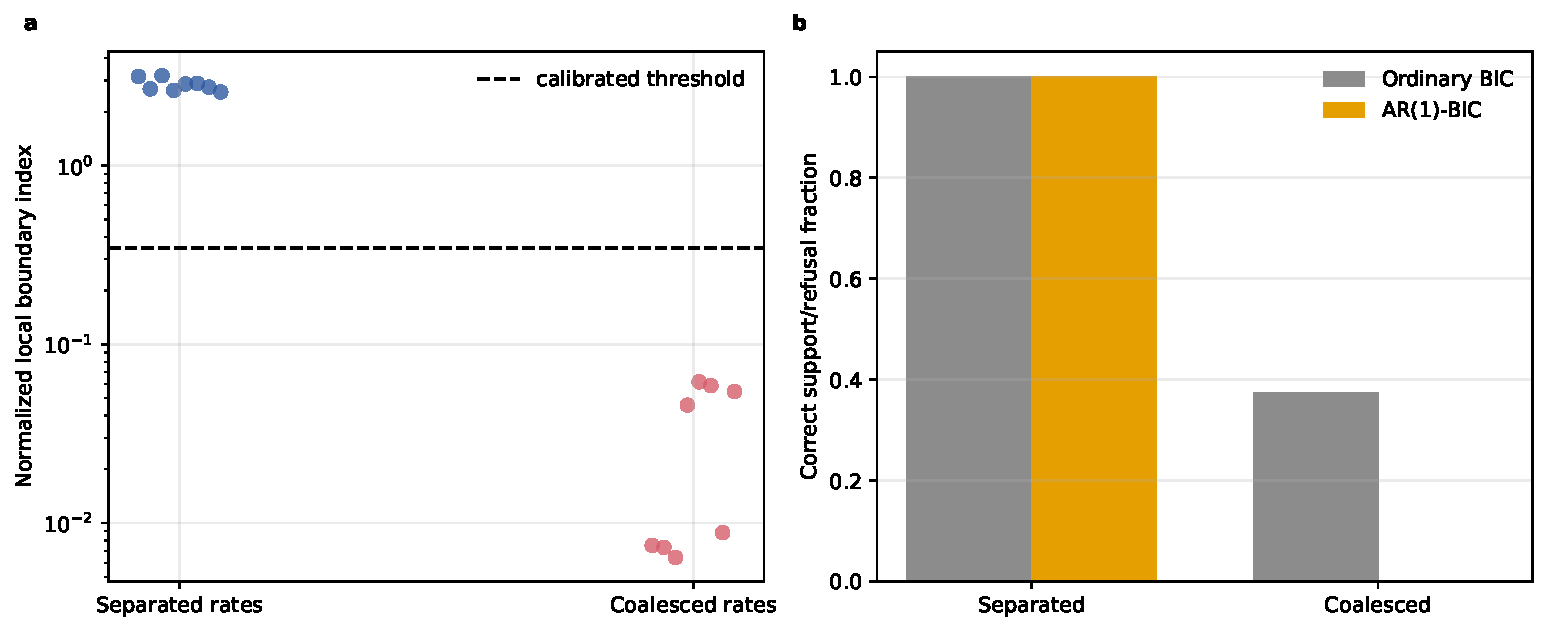
\includegraphics[width=0.90\textwidth]{fig_stage65_acceptance_calibration.pdf}
\caption{Semi-synthetic calibration with disjoint calibration and evaluation seeds. (a) The normalized local-boundary proxy separates the declared well-separated and coalesced designs. (b) Correct support or refusal under ordinary and AR(1)-profile BIC; the explicit boundary gate is needed because information criteria alone often merge unresolved nearby rates.}
\label{fig:semisynthetic}
\end{figure}

\subsection{Finite-budget resolution and matrix-pencil stability}
Information-criterion selection alone did not protect the spectral interpretation. Across 54 design cells and 1,080 independent trials, block matrix-pencil BIC selected rank two 157 times; 60 of those selections exceeded the declared log-rate error tolerance. The complete evidence gate retained 74 rank-two supports and none was inaccurate (Table~\ref{tab:resolution-atlas}). Within the tested grid, the smallest supported budget occurred only at relative noise 0.001 and adjacent log-rate gap 0.32, with horizon 8 and 24 observations per channel. No cell at the two higher noise levels or two smaller gaps supported rank two. This atlas estimates a method- and design-specific resolution region, not a universal phase boundary.

\begin{table}[H]
\centering
\caption{Finite-budget resolution atlas for block matrix-pencil recovery.}
\label{tab:resolution-atlas}
\begin{tabular}{lr}
\toprule
Quantity & Result \\
\midrule
Design cells / independent trials & 54 / 1,080 \\
Rank-two selections by BIC & 157 \\
Inaccurate BIC rank-two selections & 60 \\
Rank-two supports after evidence gating & 74 \\
Inaccurate gated supports & 0 \\
Smallest supported cell $(\sigma,\Delta\log\lambda,T,n)$ & $(0.001,0.32,8,24)$ \\
\bottomrule
\end{tabular}
\end{table}

\subsection{Common-budget power certification and order baselines}
The ungated common-budget detector frequently promoted unresolved rank-two signals to rank one. Requiring a separately calibrated design-power certificate qualified 8 of 24 observation designs. On 1,152 evaluation trials, the frozen selective rule attained coverage 0.2943, selective accuracy 0.8614, and selective risk 0.1386, with zero false order elevation and false order reduction 0.0612 (Table~\ref{tab:common-budget}). Thresholds from 0.70 through 0.90 produced the same decisions; relaxing the threshold to 0.30 increased coverage to 0.3472 but raised selective risk to 0.1900.

\begin{table}[H]
\centering
\caption{Common-budget order selection on the same 1,152 evaluation trials. Full-coverage methods cannot be compared to the selective method by accuracy alone.}
\label{tab:common-budget}
\begin{tabular}{lrrrr}
\toprule
Method & Coverage & Selective risk & False elevation & False reduction \\
\midrule
Matrix-pencil AICc & 1.0000 & 0.3559 & 0.0000 & 0.5339 \\
Block-Hankel AIC & 1.0000 & 0.3342 & 0.6771 & 0.1628 \\
Block-Hankel MDL & 1.0000 & 0.3854 & 0.2839 & 0.4362 \\
Shared-Prony AICc & 1.0000 & 0.4965 & 0.6224 & 0.4336 \\
Shared-Prony BIC & 1.0000 & 0.4983 & 0.5911 & 0.4518 \\
Power-certified selective & 0.2943 & 0.1386 & 0.0000 & 0.0612 \\
\bottomrule
\end{tabular}
\end{table}

The result supports a distinct reliability--coverage operating regime, not unconditional superiority: 70.57\% of trials abstain, and the certificate is conditional on the declared 0.32 rate gap. Block-Hankel columns overlap and are dependent, so their AIC/MDL scores are explicit subspace comparators rather than exact independent-observation likelihood criteria.

\subsection{Leave-one-gate-out decision audit}
We reapplied the decision rule to frozen stress records without refitting. PVA boundary records supplied transitions that failed only transfer or only stability; the UCI gas record supplied a transition that failed only separation; and a controlled transition with negative information gain but all other checks passing audited the information logic. Under the full contract each record refused or stayed at the lower rank. Omitting its single failed gate promoted the higher rank in all four cases. This establishes that the gates are not redundant Boolean decoration on these stress records. It is a logical relevance audit on selected records, not an estimate of population-level variable importance.
\subsection{Independent PVA support and its boundary}
On the complete 28-s task, the protocol returns \texttt{SUPPORTED\_RANK\_3}. Table~\ref{tab:pva} shows that rank three has the lowest BIC and held-curve NRMSE while remaining within the rate-stability and separation gates.

\begin{table}[H]
\centering
\caption{PVA public-data result under the frozen protocol.}
\label{tab:pva}
\begin{tabular}{rrrr}
\toprule
Rank & Mean BIC & Median held NRMSE & Max. fold log-rate SD\\
\midrule
1 & $-6944.806$ & 0.01757 & 0.0284\\
2 & $-8350.562$ & 0.01121 & 0.1540\\
3 & $-8670.737$ & 0.00932 & 0.3685\\
\bottomrule
\end{tabular}
\end{table}

Rank three improves the median curve error over rank one by 48.4\%, with a descriptive bootstrap interval of [39.5\%, 79.8\%]. The horizon-by-budget map is nonmonotone. At fixed spacing, the decision changes from rank two at 4 s, to indeterminate at 8 and 15 s, and to rank three at 28 s. Over the same sequence, median lag-one residual correlation increases from $-0.075$ to 0.400 and the rate-sensitivity condition number increases from 45.9 to 156.6. At 28 s, changing optimizer starts from one to eight does not change the decision. These observations implicate tail coverage, correlated information, and conditioning rather than a simple start-budget failure.

\begin{figure}[H]
\centering
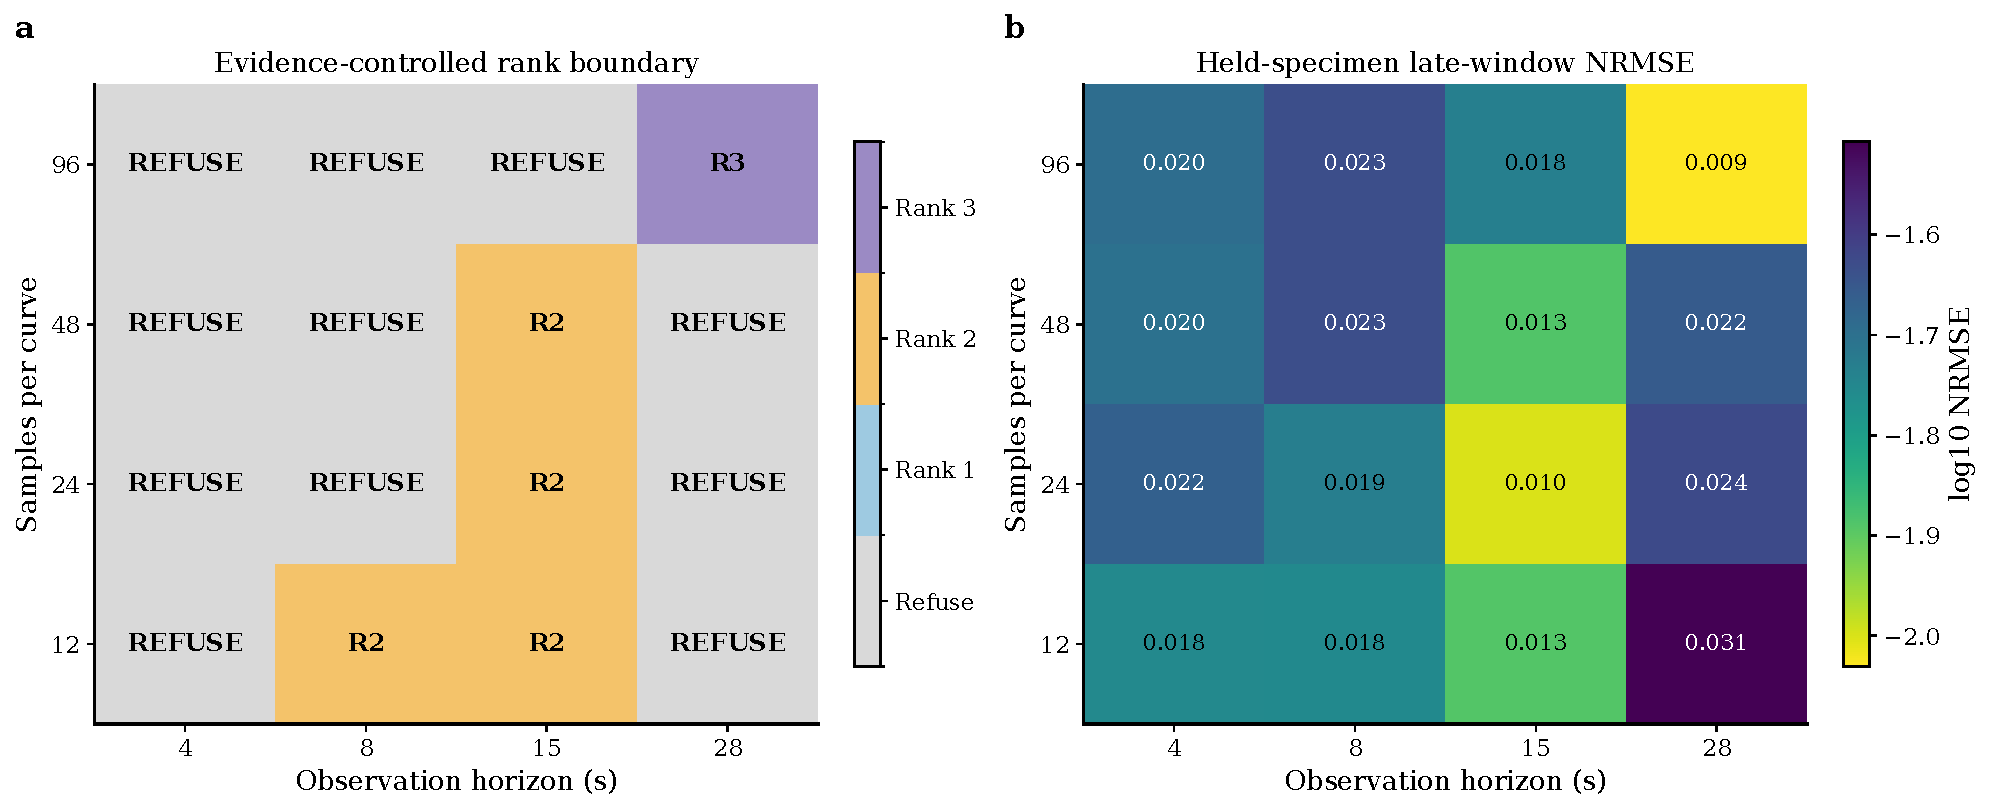
\includegraphics[width=0.94\textwidth]{fig_stage62_identifiability_boundary.pdf}
\caption{Observation-design boundary on the PVA task. The map records supported ranks and refusal regions rather than forcing a rank at every horizon and sampling budget.}
\label{fig:pva-boundary}
\end{figure}

Retrospective application of the frozen common-budget adapter to 56 groups from the four public tasks admitted only the original six-curve PVA group; 55 groups were scope-refused rather than coerced into a decision. The admitted group supplied evidence against rank-one sufficiency. Enumerating all $\binom{9}{6}=84$ overlapping PVA subsets without retuning gave the same result in every subset: all entered the 0.005 white-noise calibration cell, passed all five rank-two checks, and rejected rank-one sufficiency. Their rank-one-to-rank-two criterion improvement ranged from 491.26 to 596.22 (median 534.29). This is robustness to group composition within one retrospective dataset, not 84 independent replications and not a prospective rank-two confirmation.

The preregistered cable-ageing group independently entered the 0.005 white-noise calibration cell, with noise proxy 0.001810 and zero monotonicity violations. Its rank-one-to-rank-two criterion improvement was 647.951; all five rank-two checks passed and the unchanged rule returned evidence against rank-one sufficiency. The design certificate was not qualified for a positive rank-one claim. Across 12 post-result start/end-window settings, every window remained eligible with the same decision and criterion improvement from 399.989 to 714.271. These overlapping windows are sensitivity checks, not independent replications. The transfer was frozen before its P5 outcome, but prior P3 use prevents treating it as investigator-blind prospective confirmation.

\subsection{Copper-alloy support with residual-model sensitivity}
Across 17 independent stress-relaxation tests and nine held material groups, AR(1)-profile BIC supports a shared rank-one empirical realization. Table~\ref{tab:kupfer} shows that adding modes reduces ordinary residual BIC but worsens held-group prediction sharply; the residual-aware criterion and the predictive gate therefore agree on rank one. The ordinary-BIC preference for richer ranks is retained as a sensitivity result rather than hidden.

\begin{table}[H]
\centering
\caption{KupferDigital leave-one-material-group-out audit. Lower held NRMSE is better.}
\label{tab:kupfer}
\begin{tabular}{rrrr}
\toprule
Rank & Mean BIC & Mean AR(1)-BIC & Median held NRMSE\\
\midrule
1 & $-13217.40$ & $-16539.53$ & 0.3845\\
2 & $-14343.85$ & $-16512.92$ & 1.7611\\
3 & $-14468.55$ & $-16432.65$ & 104.2460\\
\bottomrule
\end{tabular}
\end{table}

The selected rate is 3.8989 h$^{-1}$. Its foldwise log-rate standard deviation is 0.7148, within the frozen stability limit of 0.8. This result supports a compact shared empirical relaxation state over the declared registered curves. It does not identify a unique microscopic copper-alloy relaxation mechanism.

\subsection{Gas-sensor prediction and refusal}
The shared rank-three model is predictively competitive on the gas-sensor recovery task (Table~\ref{tab:gas}). It improves the median experiment error by 26.6\% relative to independent nonlinear fitting ($p=0.00110$), 80.6\% relative to fixed-grid NNLS ($p<10^{-12}$), and 8.25\% relative to Prony recurrence ($p=0.00928$).

\begin{table}[H]
\centering
\caption{Held-experiment prediction on 50 non-air gas exposures.}
\label{tab:gas}
\begin{tabular}{lcc}
\toprule
Method & Median NRMSE & Interquartile range\\
\midrule
Shared rank 3 & 0.05392 & [0.03420, 0.07168]\\
Independent nonlinear rank 3 & 0.05910 & [0.05189, 0.07471]\\
Fixed-grid NNLS & 0.25676 & [0.20728, 0.31036]\\
Prony recurrence & 0.05961 & [0.03894, 0.08373]\\
\bottomrule
\end{tabular}
\end{table}

Nevertheless, two fitted rank-three rates coalesce near $0.03765$, violating Eq.~\eqref{eq:separation}. The protocol therefore returns \indet{}. Rank three versus rank one yields a median experiment-level prediction improvement of 65.9\%, with a clustered-bootstrap 95\% interval of [58.5\%, 68.2\%], yet this predictive gain does not repair spectral non-identifiability. All 27 threshold combinations remain \indet{}, and 2/4/8-start fits return the same objective and rates.

\begin{figure}[H]
\centering
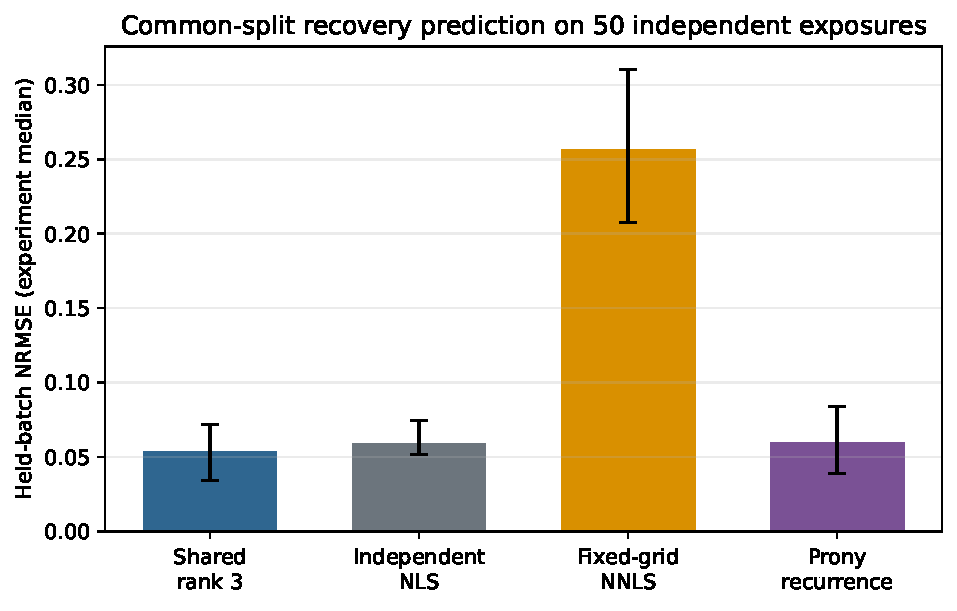
\includegraphics[width=0.94\textwidth]{fig_stage63_external_baselines.pdf}
\caption{Matched external baselines on the gas-sensor task. Points are independent exposure experiments; sensor channels are not counted as independent replicates.}
\label{fig:baselines}
\end{figure}

\begin{figure}[H]
\centering
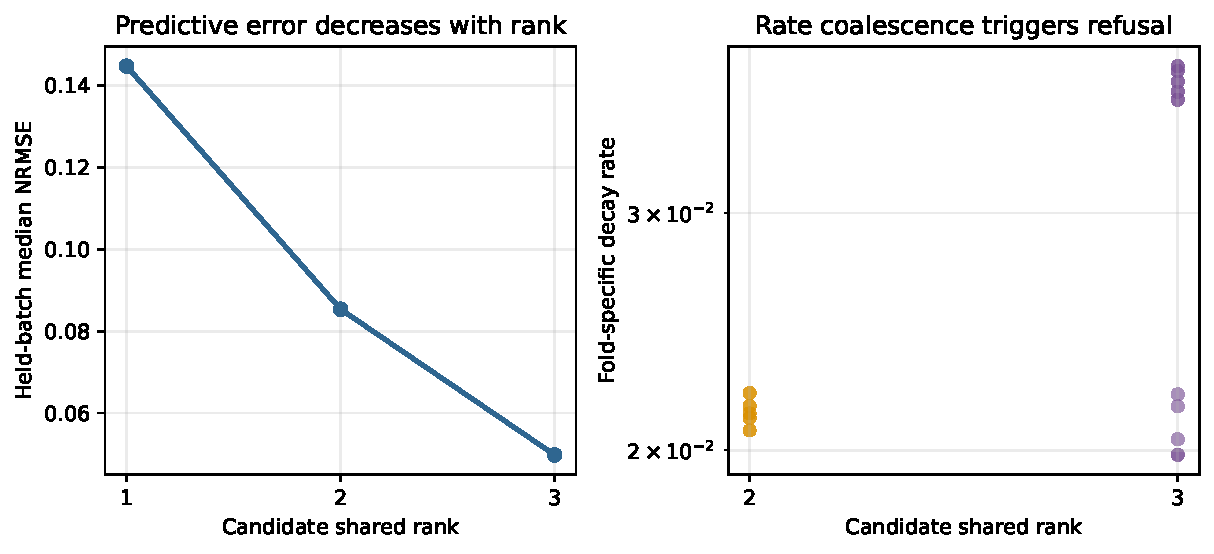
\includegraphics[width=0.94\textwidth]{fig_stage63_rank_refusal.pdf}
\caption{Predictive improvement and the refusal decision. The shared rank-three fit predicts well, but the rate-separation gate prevents a three-timescale mechanism claim.}
\label{fig:refusal}
\end{figure}

\subsection{Hydraulic-state transfer exposes a second refusal mode}
On the hydraulic task, rank two improves mean BIC from $-8509.645$ to $-9167.872$, but median held-cycle NRMSE worsens from 0.23780 to 0.51128. The median rank-two relative improvement is therefore $-73.5\%$ across 30 independent cycles (cluster-bootstrap 95\% interval $[-144.0\%,-38.4\%]$). Its fitted rates collapse at the lower bound and its local boundary index is 0.0571. Rank three also fails: held-cycle NRMSE is 0.42922, all three full-data rates coalesce near 0.069, and the boundary index is $1.85\times10^{-7}$. The decision is \indet{} for all 27 threshold combinations. Correlation sensitivity strengthens rather than reverses the refusal: ordinary BIC favors rank two, whereas AR(1)-profile BIC is lowest for rank one ($-10208.35$, compared with $-9936.23$ for rank two and $-9532.14$ for rank three). The corresponding mean residual AR(1) estimates decrease from 0.68 to 0.49 and 0.40.

 For the three gas baselines, Holm-adjusted one-sided paired values are $2.66\times10^{-15}$ (fixed-grid NNLS), 0.00220 (independent nonlinear rank three), and 0.00928 (Prony); the matched predictive conclusions therefore survive within-task multiplicity correction.

This refusal differs from the gas result. Gas recovery shows predictive benefit without spectral separation; the hydraulic task shows in-sample information improvement without held-condition transfer or separation. The two cases exercise different terms of the evidence contract.

Matched early-to-late model-family controls also rule out a trivial weak-baseline explanation. At the independent-cycle level, the shared rank-one model has median NRMSE 0.244, compared with 0.329 for a stretched exponential, 0.316 for AR(2), 0.491 for Prony recurrence, and 0.625 for fixed-grid NNLS. Within the four hydraulic baseline comparisons, Holm-adjusted paired Wilcoxon values are $7.98\times10^{-4}$ for the stretched exponential, $6.48\times10^{-6}$ for Prony, $1.20\times10^{-5}$ for NNLS, and 0.0249 for AR(2). The AR(2) bootstrap interval for the paired median difference crosses zero, so that comparison remains mixed despite its adjusted rank-test value. These controls establish predictive competitiveness on the declared transient window, not component-level physical mechanism identification.

\begin{figure}[H]
\centering
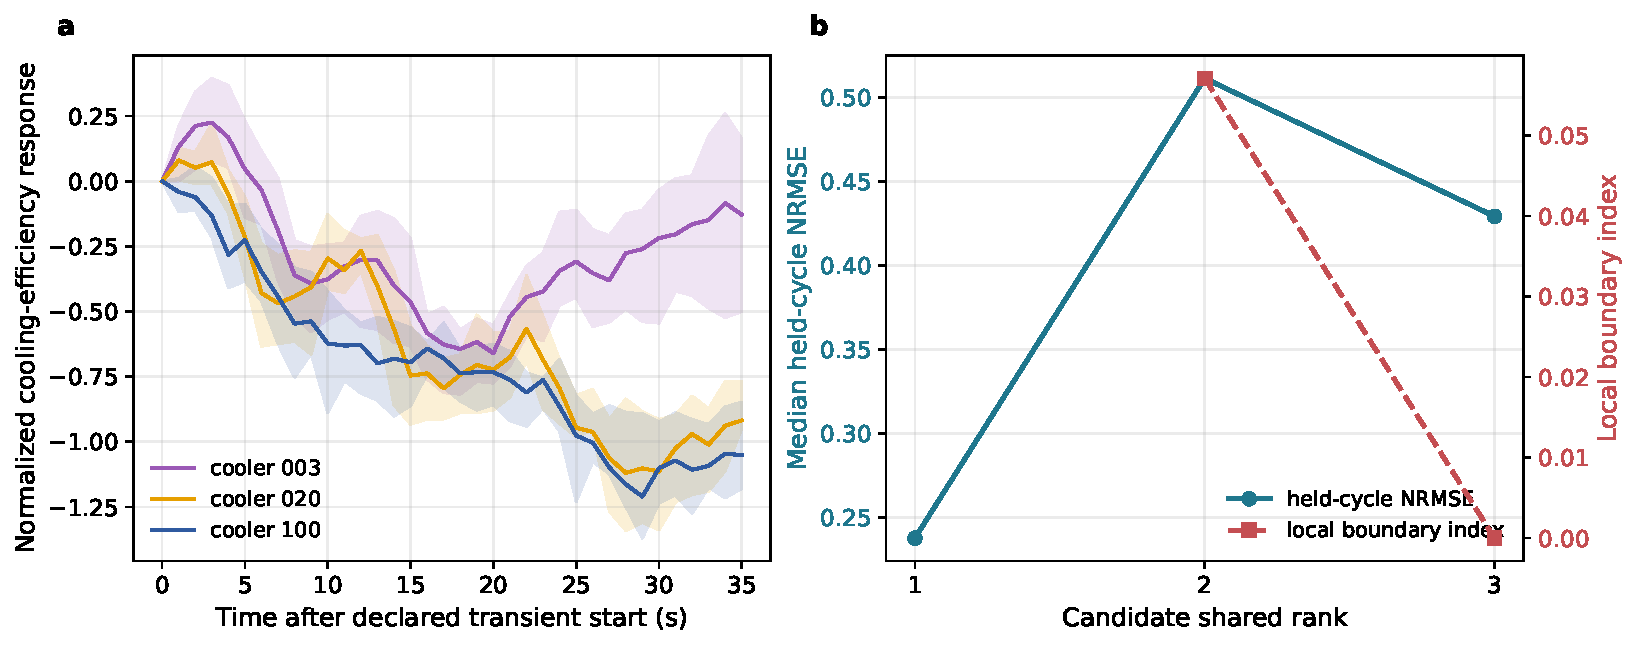
\includegraphics[width=0.96\textwidth]{fig_stage64_hydraulic_transients.pdf}
\caption{Third-domain hydraulic audit. (a) Normalized cooling-efficiency transients across controlled cooler states; bands show interquartile ranges over independent cycles. (b) Held-cycle prediction error and the projected-sensitivity boundary diagnostic. The latter is a within-rank identifiability indicator, not a cross-rank performance score.}
\label{fig:hydraulic}
\end{figure}

\subsection{Controlled tests of the recommended extension combination}
Four controlled audits used 12 independent seeds (Fig.~\ref{fig:extensions}). For damped oscillations, replacing three positive real poles with one stable conjugate pair reduced median held-horizon NRMSE from 0.12102 to 0.002079, a 98.3\% relative reduction (one-sided paired Wilcoxon $p=2.44\times10^{-4}$), and recovered damping 0.16 and frequency 2.2 within numerical tolerance. Under declared group drift, partial pooling reduced median NRMSE from 0.04806 to 0.004249 (91.2\%; $p=2.44\times10^{-4}$). On dense log-normal relaxation spectra, a 32-point nonnegative grid improved over a rank-three finite fit by a median 59.3\%; the predeclared 20\% mismatch threshold refused a finite-mechanism claim in 11 of 12 seeds. This comparison diagnoses finite-model-class inadequacy; it does not identify the generating spectrum. With 39 independent calibration groups, the group-conformal audit produced a 5.0\% mean false-alarm rate on exchangeable controls and 100\% empirical detection on the constructed shifted alternative. The latter is a power observation, whereas the coverage statement applies only to the exchangeable control design.

\begin{figure}[H]
\centering
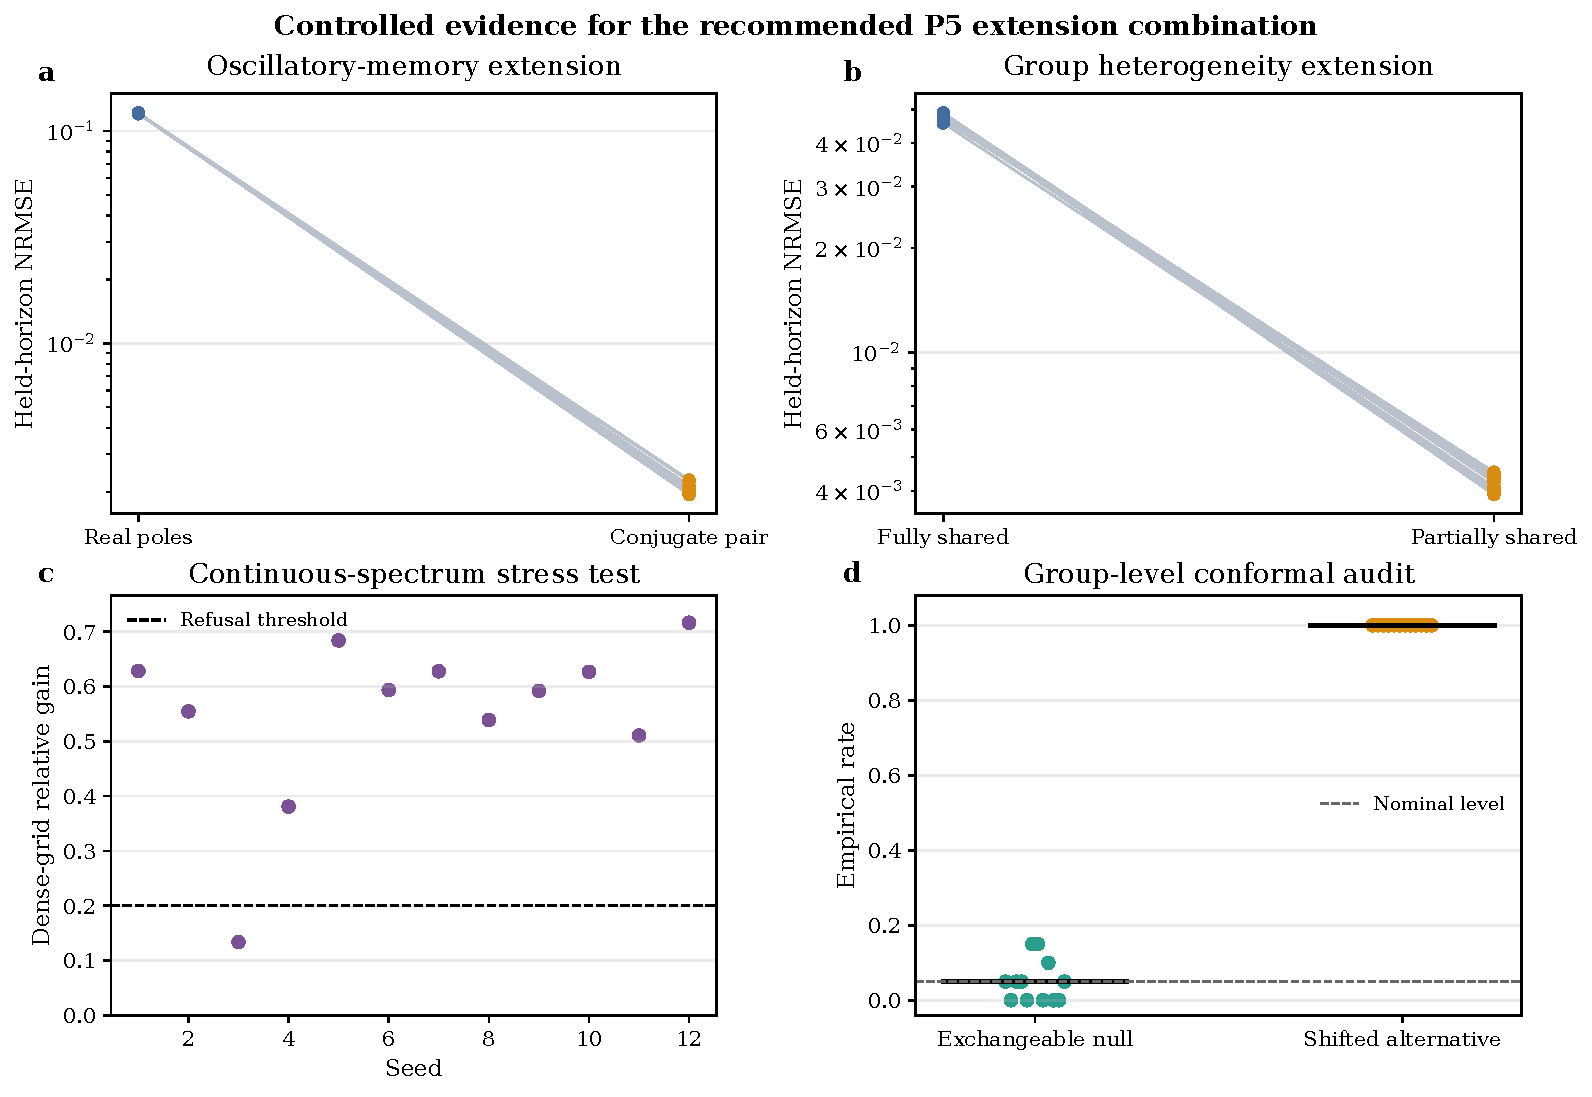
\includegraphics[width=0.96\textwidth]{fig_stage66_extension_combination.pdf}
\caption{Controlled extension audits. (a) Positive-real-pole and conjugate-pair extrapolation on damped oscillations. (b) Fully shared and partially shared rates under group heterogeneity. (c) Dense-spectrum gain over a rank-three finite model; the dashed line is the declared mismatch threshold. (d) Group-level conformal false-alarm and shifted-alternative detection rates. Panels compare only methods within the same controlled task.}
\label{fig:extensions}
\end{figure}
\section{Discussion}
The experiments establish a distinction between approximation quality and mechanism support. On PVA, cross-specimen prediction, information gain, rate stability, and separation agree at the full observation horizon. On the copper-alloy task, held-material prediction and residual-aware model selection support a shared rank-one empirical state, while ordinary BIC alone would over-rank the response. On the gas task, prediction favors a richer model but separation rejects its mechanistic interpretation. On the hydraulic task, BIC favors extra modes while transfer and separation reject them. A workflow that reports only the best in-sample or predictive rank would erase these different outcomes.

The nonmonotone PVA boundary also cautions against equating longer records or denser grids with monotonically stronger evidence. Additional tail coverage can expose a slow mode, but correlated residuals reduce effective information and an enlarged rate range can worsen conditioning. The boundary-factor audit is explanatory rather than causal; its purpose is to identify which assumptions should be tested before interpreting a rank transition.

The finite-budget atlas makes this warning operational. Matrix-pencil BIC produced 60 inaccurate rank-two recoveries among 157 rank-two selections, despite using a standard spectral estimator. Agreement across Hankel aspect ratios removed these unstable interpretations when combined with separation and local-information gates, while retaining 74 accurate supports. The absence of support at moderate noise or small rate gaps is equally informative: more samples within the tested horizon did not create spectral resolution when differencing noise and pencil conditioning dominated. The zero observed inaccurate gated supports is limited to 1,080 trials under the declared generator and tolerance; it is not a zero-risk guarantee.

The common-budget comparison quantifies the cost of protecting a rank-one statement. Full-coverage criteria exchange false elevation for false reduction, whereas the power-certified rule removes observed false elevation and sharply reduces false reduction only by abstaining on most trials. Its 0.1386 selective risk must therefore be read together with 0.2943 coverage. The low 1/56 eligibility in retrospective public-task transfer further shows that calibration scope, rather than favorable outcomes, limits reuse. PVA subset stability removes one composition artifact, while the preregistered cable-ageing transfer adds a second eligible public dataset without threshold changes and stays decision-stable across 12 post-result windows. Neither overlapping sensitivity audit is an independent replication, and prior P3 use means the cable result cannot substitute for an independently collected prospective dataset.

The gate ablation also clarifies the protocol architecture: each evidence gate blocks a distinct unsupported promotion on at least one frozen stress record, although this diagnostic does not quantify its importance in an unseen population. The protocol is deliberately narrower than a general memory-kernel learner. It assumes a declared common time grid, positive real rates, finite sums of decays, and grouped experimental units. The main model permits signed curve-specific amplitudes, which can represent channel reversals but can also create cancellation. A nonnegative-amplitude semi-synthetic ablation leaves the separated-support and coalesced-refusal findings unchanged; this does not establish equivalence on arbitrary data. The public-data decisions still do not cover irregular grids or nonlinear state-dependent memory. Controlled extensions now establish computational feasibility for stable conjugate-pole blocks, partially shared positive rates, and explicit refusal under a dense relaxation spectrum; they do not establish real-data identifiability or universal calibration for these broader classes. In higher-dimensional operator settings, the main costs move from scalar nonlinear fitting to repeated matrix-function actions and independent reference construction. A credible extension must budget reference error and preserve groupwise validation rather than merely scaling the current optimizer.

Three warning signs should trigger refusal or a weaker representation claim: adjacent rates below calibrated resolution, residual correlation that changes criterion ordering, and held-unit deterioration despite lower training error. Nonnormality and latent-parameter nonidentifiability can amplify them; higher-dimensional extensions must budget independent references and grouped holdouts. A supported realization is a compact predictive state model, not automatic proof of distinct microscopic processes. Conversely, \indet{} says only that the frozen observation contract cannot resolve the mechanism.

\section{Software and reproducibility}
The package \texttt{p5\_memory\_protocol} freezes four public operations: \texttt{fit}, \texttt{evaluate}, \texttt{decide}, and \texttt{report}. Versioned JSON records store the declared domain, grouping unit, thresholds, diagnostics, decision, and scope limits. The command
\begin{verbatim}
python -m p5_memory_protocol reproduce --task uci-gas
\end{verbatim}
replays the public gas task. At manuscript assembly, 190 unit tests passed and 85 machine-readable result files parsed successfully. These checks establish internal reproducibility; independent external reproduction remains a separate requirement.

\section{Conclusion}
We presented an evidence-gated method that identifies the smallest supported shared finite-memory realization or refuses a rank claim. The adjacent-rate boundary and its calibrated corollary delimit possible guarantees. In 1,080 finite-budget trials, the complete gate retained 74 accurate matrix-pencil supports and no inaccurate support under the declared design. In 1,152 separate common-budget trials, power certification gave 0.2943 coverage, 0.1386 selective risk, and zero observed false elevation, while five full-coverage criteria exposed directional errors. Four established public domains, all 84 PVA subsets, and frozen-rule transfers demonstrate complementary decisions, narrow cross-task scope, and within-dataset stability. The preregistered new-to-P5 cable transfer adds a second eligible dataset without retuning but is not prospectively acquired. The result is a scoped statistical signal-processing procedure, not an unconditional full-coverage order classifier.

\section*{Data and code availability}
The public source datasets are identified by DOI in the references. Derived results, protocol definitions, tests, and figure-generation scripts are available at \url{https://github.com/hzhooning-art/DFSC}. The frozen software and reproducibility archive is available at \url{https://doi.org/10.5281/zenodo.22168774}.

\section*{CRediT authorship contribution statement}
\textbf{Haitao Duan:} Conceptualization, Methodology, Software, Formal analysis, Investigation, Validation, Writing--original draft, Writing--review and editing. \textbf{Ning Hu:} Conceptualization, Methodology, Supervision, Data curation, Validation, Visualization, Writing--review and editing. \textbf{Shuqun Li:} Investigation, Validation, Formal analysis, Writing--review and editing. \textbf{Chuyang Hu:} Investigation, Validation, Software verification, Writing--review and editing.

\section*{Funding}
This work was supported by the State Key Laboratory of Ocean Engineering, Shanghai Jiao Tong University (Grant No. GKZD010089), and the State Key Laboratory of Acoustics, Chinese Academy of Sciences (Grant No. SKLA202406). The funders had no role in the study design; collection, analysis, and interpretation of data; writing of the manuscript; or decision to submit the article for publication.

\section*{Declaration of competing interest}
The authors declare that they have no known competing financial interests or personal relationships that could have appeared to influence the work reported in this paper.

\section*{Declaration of generative AI and AI-assisted technologies}
During manuscript preparation, the authors used AI-assisted tools for language editing, document organization, and consistency checks. The authors reviewed and verified the resulting text, numerical claims, code outputs, and references and take full responsibility for the manuscript.

\section*{Ethics statement}
This study uses public non-human datasets and synthetic numerical experiments. No human participants, identifiable personal data, or animal experiments were involved.

\section*{Author identifiers}
Haitao Duan: ORCID 0009-0006-4611-8639; Ning Hu: ORCID 0000-0002-2718-0385; Shuqun Li: ORCID 0009-0007-1787-685X; Chuyang Hu: ORCID 0009-0007-9255-018X.

\bibliographystyle{unsrt}
\bibliography{references}
\end{document}






